\documentclass[12pt,a4paper]{article}

\usepackage[a4paper,margin=1in]{geometry}
\usepackage{graphicx}
\usepackage{booktabs}
\usepackage{amsmath,amssymb}
\usepackage{float}
\usepackage{hyperref}
\usepackage{xcolor}
\usepackage{enumitem}
\usepackage{fancyhdr}
\usepackage{longtable}

\hypersetup{colorlinks=true,linkcolor=blue,urlcolor=blue}

\pagestyle{fancy}
\fancyhf{}
\lhead{ICS1512}
\rhead{Machine Learning Algorithms Laboratory}
\cfoot{\thepage}

\begin{document}

\begin{tabular}{|p{4cm}|p{11cm}|}
\hline
Experiment No. & 2 \\ \hline
Experiment Title &
Email Spam Detection using KNN and Naive Bayes Classifiers
\footnote{\textbf{GitHub Repository: }\url{https://github.com/JJBOY12345/MLAssign_SSN}}\\ \hline
Student Name & \\ \hline
Register Number & \\ \hline
Faculty & Dr. Poreddy Ajay Kumar Reddy \\ \hline
Submission Date & \\ \hline
\end{tabular}

\section{Objective}
TODO: State the objective of this experiment — to classify emails as spam or ham using K-Nearest Neighbors (KNN) and three variants of Naive Bayes (Gaussian, Multinomial, Bernoulli), and to compare their performance using various evaluation metrics.

\section{Problem Statement}
TODO: Describe the problem — given a dataset of email word frequencies, the task is to predict whether an email is spam (1) or ham (0). Discuss the input (word frequency features), output (binary classification), and objective (accurate spam detection).

\section{Dataset Description}
\begin{longtable}{|p{5cm}|p{9cm}|}
\hline
Dataset Name & Spambase \\ \hline
Dataset Source & \texttt{spamEmail/spambase\_csv.csv} (UCI Repository) \\ \hline
Number of Samples & 4,601 \\ \hline
Number of Features & 57 (word frequency columns) + 1 target (class) \\ \hline
Number of Classes & 2 (Spam / Ham) \\ \hline
Missing Values & None \\ \hline
Duplicate Records & 391 \\ \hline
Train-Test Split & 80\% Train, 20\% Test (stratified) \\ \hline
\end{longtable}

TODO: Describe the dataset, its features, and the classification task.

\section{Exploratory Data Analysis}
For the Spambase dataset, only class distribution was plotted (histograms, box plots, heatmap, and pair plot were intentionally skipped due to the high dimensionality of the data).

\subsection{Class Distribution}
\begin{figure}[H]
\centering

\includegraphics[width=0.7\linewidth]{images/spam_class_distribution.png}
\caption{Class Distribution of Spam vs Ham Emails}
\end{figure}

\textbf{Inference:}
TODO: Discuss the balance (or imbalance) between spam and non-spam classes.

\section{Data Preprocessing}
Explain the preprocessing steps performed:
\begin{itemize}
    \item \textbf{Feature-Target Separation}: Features (X) and target (y) were separated.
    \item \textbf{Train-Test Split}: Data was split into 80\% training and 20\% testing using stratified sampling.
    \item \textbf{Standard Scaling}: \texttt{StandardScaler} was applied for KNN and Gaussian NB.
    \item \textbf{Min-Max Scaling}: \texttt{MinMaxScaler} was applied for Multinomial NB and Bernoulli NB.
\end{itemize}

\section{Machine Learning Algorithms}
Explain the working principle, mathematical formulation, advantages, and limitations of each algorithm used:

\subsection{K-Nearest Neighbors (KNN)}
TODO: Explain KNN — instance-based learning, Euclidean distance, choice of k, majority voting.

\subsection{Gaussian Naive Bayes}
TODO: Explain Gaussian NB — assumes features follow a normal distribution, suitable for continuous data.

\subsection{Multinomial Naive Bayes}
TODO: Explain Multinomial NB — suitable for discrete count data (word frequencies), requires non-negative features.

\subsection{Bernoulli Naive Bayes}
TODO: Explain Bernoulli NB — suitable for binary/boolean features, works with binarized data.

\section{Experimental Setup}
\begin{tabular}{ll}
\toprule
Python Version & TODO: Specify \\
Scikit-Learn Version & TODO: Specify \\
IDE & TODO: Specify \\
Operating System & TODO: Specify \\
Hardware & TODO: Specify \\
\bottomrule
\end{tabular}

\section{Model 1: K-Nearest Neighbors (KNN)}

\subsection{Hyperparameter Selection — K Value}
The performance of KNN was evaluated for odd values of k from 1 to 29.

\begin{figure}[H]
\centering
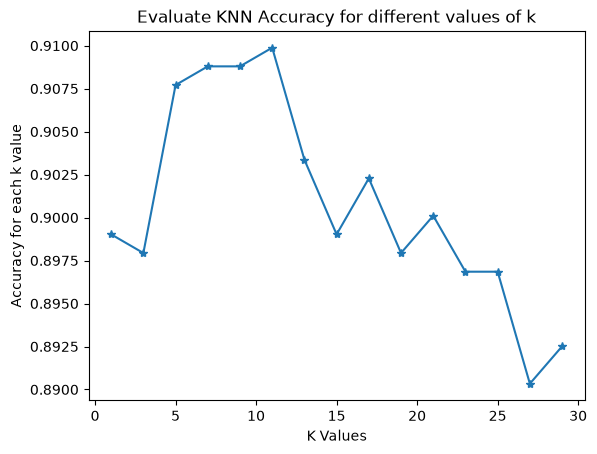
\includegraphics[width=0.7\linewidth]{images/knn_accuracy_vs_k.png}
\caption{Accuracy vs K Value for KNN}
\end{figure}

\textbf{Inference:}
TODO: Discuss how accuracy varies with k, identify the optimal k value.

\begin{table}[H]
\centering
\begin{tabular}{lcccc}
\toprule
\textbf{k} & \textbf{Accuracy} & \textbf{Precision} & \textbf{Recall} & \textbf{F1-Score} \\ \midrule
1 & 0.899 & 0.895 & 0.893 & 0.894 \\
3 & 0.898 & 0.893 & 0.893 & 0.893 \\
5 & 0.908 & 0.904 & 0.903 & 0.903 \\
7 & 0.909 & 0.906 & 0.903 & 0.904 \\
9 & 0.909 & 0.906 & 0.903 & 0.904 \\
11 & 0.910 & 0.908 & 0.903 & 0.905 \\
\bottomrule
\end{tabular}
\caption{Performance Metrics for Different K Values}
\end{table}

\subsection{Hyperparameter Tuning — GridSearchCV}
TODO: Explain GridSearchCV — parameter grid \{n\_neighbors, metric, weights\}, 5-fold CV.

\begin{longtable}{|l|l|}
\hline
\textbf{Parameter} & \textbf{Values Searched} \\ \hline
n\_neighbors & 1, 3, 5, 7, 9, 11, 13, 15 \\ \hline
metric & euclidean, manhattan \\ \hline
weights & uniform, distance \\ \hline
\end{longtable}

TODO: Report best parameters and best CV score.

\subsection{Hyperparameter Tuning — RandomizedSearchCV}
TODO: Explain RandomizedSearchCV with the same parameter space, n\_iter=10.

TODO: Report best parameters and best CV score from RandomizedSearchCV.

\subsection{KDTree vs BallTree Comparison}
TODO: Compare the performance of KNN using KDTree and BallTree algorithms in terms of accuracy and training/testing time.

\begin{table}[H]
\centering
\begin{tabular}{lccc}
\toprule
\textbf{Algorithm} & \textbf{Accuracy} & \textbf{Train Time (s)} & \textbf{Test Time (s)} \\ \midrule
KDTree & TODO & TODO & TODO \\
BallTree & TODO & TODO & TODO \\
\bottomrule
\end{tabular}
\caption{KDTree vs BallTree Performance Comparison}
\end{table}

\section{Model 2: Gaussian Naive Bayes}
TODO: Explain the training process using StandardScaled features.

\subsection{Results}
\begin{table}[H]
\centering
\begin{tabular}{lc}
\toprule
\textbf{Metric} & \textbf{Value} \\ \midrule
Accuracy & 0.833 \\
Precision & 0.84 (macro avg) \\
Recall & 0.85 (macro avg) \\
F1-Score & 0.84 (macro avg) \\
ROC-AUC & 0.938 \\
\bottomrule
\end{tabular}
\caption{Gaussian NB Performance Metrics}
\end{table}

\subsection{Confusion Matrix}
\begin{figure}[H]
\centering
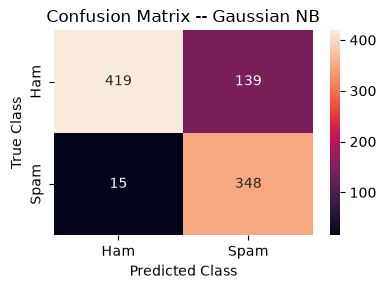
\includegraphics[width=0.6\linewidth]{images/gaussianNB_confusion_matrix.png}
\caption{Confusion Matrix — Gaussian NB}
\end{figure}

\textbf{Inference:}
TODO: Interpret the confusion matrix — true positives, false positives, etc.

\subsection{ROC Curve}
\begin{figure}[H]
\centering
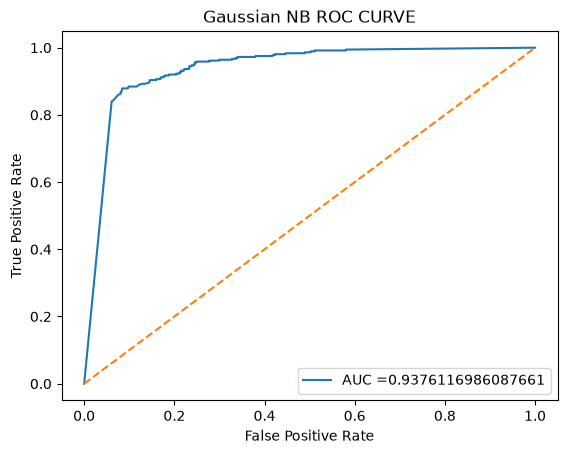
\includegraphics[width=0.6\linewidth]{images/gaussianNB_roc_curve.png}
\caption{ROC Curve — Gaussian NB}
\end{figure}

\textbf{Inference:}
TODO: Discuss the ROC-AUC score and what it indicates about model performance.

\subsection{Precision-Recall Curve}
\begin{figure}[H]
\centering
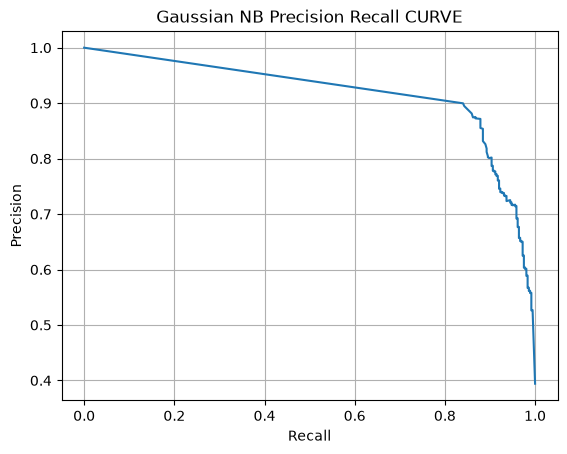
\includegraphics[width=0.6\linewidth]{images/gaussianNB_pr_curve.png}
\caption{Precision-Recall Curve — Gaussian NB}
\end{figure}

\textbf{Inference:}
TODO: Discuss the precision-recall trade-off observed.

\subsection{Cross-Validation}
\begin{figure}[H]
\centering
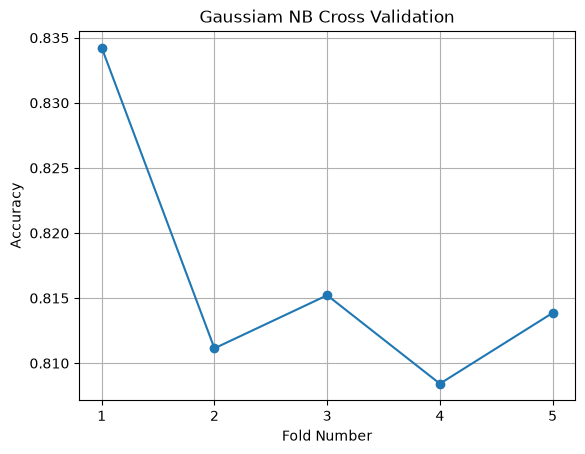
\includegraphics[width=0.6\linewidth]{images/gaussianNB_cross_validation.png}
\caption{5-Fold Cross-Validation — Gaussian NB}
\end{figure}

\textbf{Inference:}
TODO: Discuss the fold accuracies and mean accuracy (0.817).

\section{Model 3: Multinomial Naive Bayes}
TODO: Explain the training process using MinMaxScaled features.

\subsection{Results}
\begin{table}[H]
\centering
\begin{tabular}{lc}
\toprule
\textbf{Metric} & \textbf{Value} \\ \midrule
Accuracy & 0.896 \\
Precision & 0.91 (macro avg) \\
Recall & 0.88 (macro avg) \\
F1-Score & 0.89 (macro avg) \\
ROC-AUC & 0.961 \\
\bottomrule
\end{tabular}
\caption{Multinomial NB Performance Metrics}
\end{table}

\subsection{Confusion Matrix}
\begin{figure}[H]
\centering
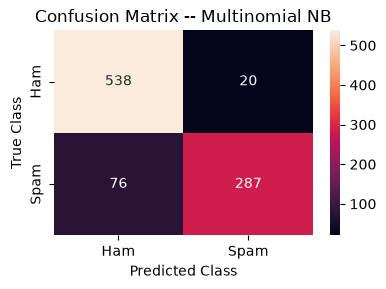
\includegraphics[width=0.6\linewidth]{images/multinomialNB_confusion_matrix.png}
\caption{Confusion Matrix — Multinomial NB}
\end{figure}

\textbf{Inference:}
TODO: Interpret the confusion matrix.

\subsection{ROC Curve}
\begin{figure}[H]
\centering
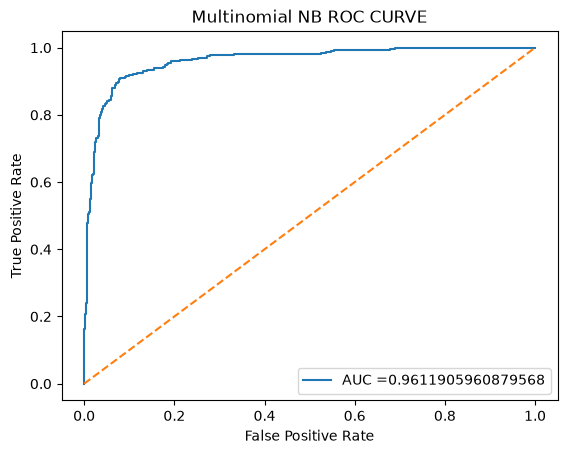
\includegraphics[width=0.6\linewidth]{images/multinomialNB_roc_curve.png}
\caption{ROC Curve — Multinomial NB}
\end{figure}

\textbf{Inference:}
TODO: Discuss the ROC-AUC score.

\subsection{Precision-Recall Curve}
\begin{figure}[H]
\centering
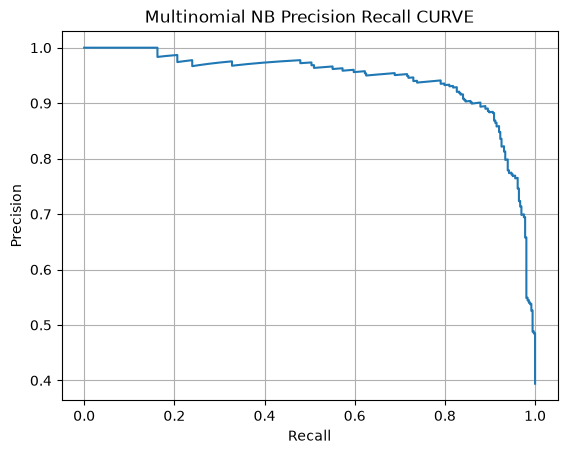
\includegraphics[width=0.6\linewidth]{images/multinomialNB_pr_curve.png}
\caption{Precision-Recall Curve — Multinomial NB}
\end{figure}

\textbf{Inference:}
TODO: Discuss the precision-recall trade-off.

\subsection{Cross-Validation}
\begin{figure}[H]
\centering
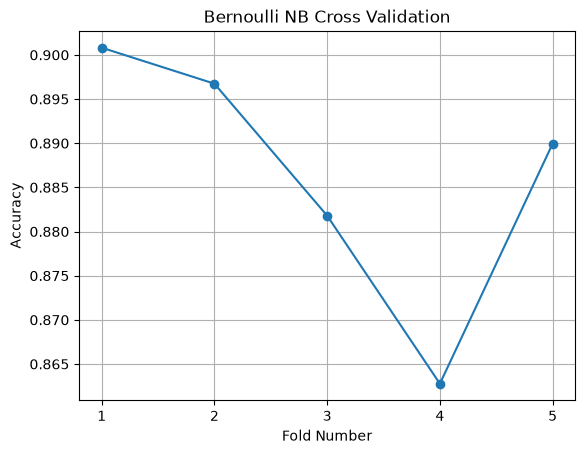
\includegraphics[width=0.6\linewidth]{images/multinomialNB_cross_validation.png}
\caption{5-Fold Cross-Validation — Multinomial NB}
\end{figure}

\textbf{Inference:}
TODO: Discuss the fold accuracies and mean accuracy (0.788).

\section{Model 4: Bernoulli Naive Bayes}
TODO: Explain the training process using MinMaxScaled features.

\subsection{Results}
\begin{table}[H]
\centering
\begin{tabular}{lc}
\toprule
\textbf{Metric} & \textbf{Value} \\ \midrule
Accuracy & 0.879 \\
Precision & 0.88 (macro avg) \\
Recall & 0.87 (macro avg) \\
F1-Score & 0.88 (macro avg) \\
ROC-AUC & 0.946 \\
\bottomrule
\end{tabular}
\caption{Bernoulli NB Performance Metrics}
\end{table}

\subsection{Confusion Matrix}
\begin{figure}[H]
\centering
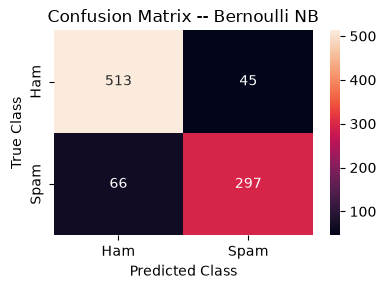
\includegraphics[width=0.6\linewidth]{images/bernoulliNB_confusion_matrix.png}
\caption{Confusion Matrix — Bernoulli NB}
\end{figure}

\textbf{Inference:}
TODO: Interpret the confusion matrix.

\subsection{ROC Curve}
\begin{figure}[H]
\centering
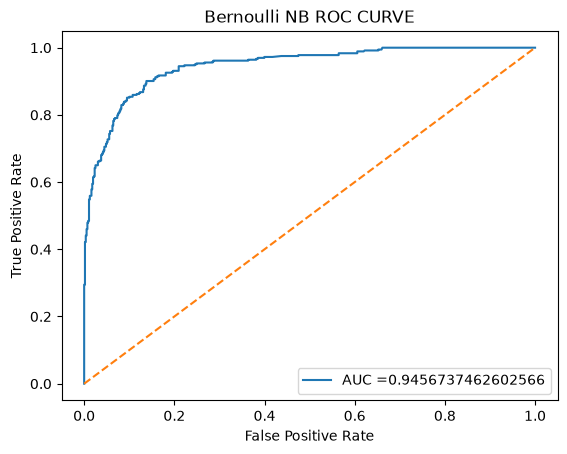
\includegraphics[width=0.6\linewidth]{images/bernoulliNB_roc_curve.png}
\caption{ROC Curve — Bernoulli NB}
\end{figure}

\textbf{Inference:}
TODO: Discuss the ROC-AUC score.

\subsection{Precision-Recall Curve}
\begin{figure}[H]
\centering
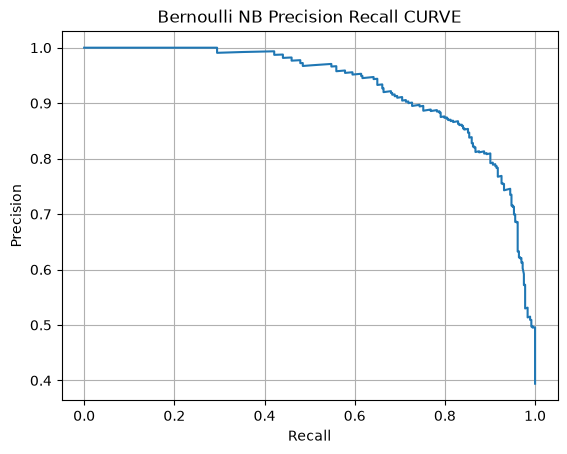
\includegraphics[width=0.6\linewidth]{images/bernoulliNB_pr_curve.png}
\caption{Precision-Recall Curve — Bernoulli NB}
\end{figure}

\textbf{Inference:}
TODO: Discuss the precision-recall trade-off.

\subsection{Cross-Validation}
\begin{figure}[H]
\centering
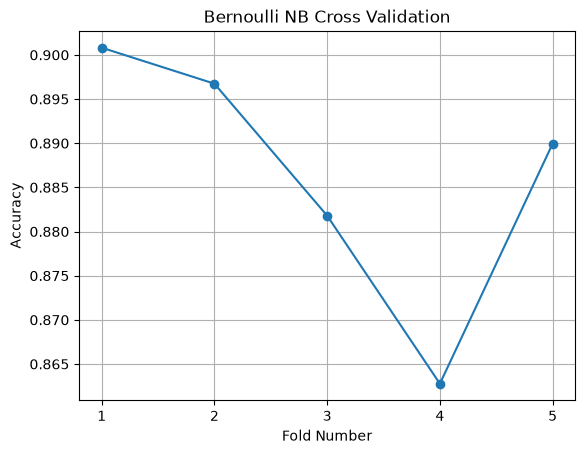
\includegraphics[width=0.6\linewidth]{images/bernoulliNB_cross_validation.png}
\caption{5-Fold Cross-Validation — Bernoulli NB}
\end{figure}

\textbf{Inference:}
TODO: Discuss the fold accuracies and mean accuracy (0.886).

\section{5-Fold Cross-Validation Comparison}
\begin{table}[H]
\centering
\begin{tabular}{lccc}
\toprule
\textbf{Model} & \textbf{Mean CV Accuracy} & \textbf{Avg Train Time (s)} & \textbf{Avg Predict Time (s)} \\ \midrule
KNN (k=11) & TODO & TODO & TODO \\
Gaussian NB & 0.817 & TODO & TODO \\
Multinomial NB & 0.788 & TODO & TODO \\
Bernoulli NB & 0.886 & TODO & TODO \\
\bottomrule
\end{tabular}
\caption{5-Fold Cross-Validation Results Across All Models}
\end{table}

\section{Result Visualization}

\subsection{Confusion Matrices Comparison}
\begin{figure}[H]
\centering
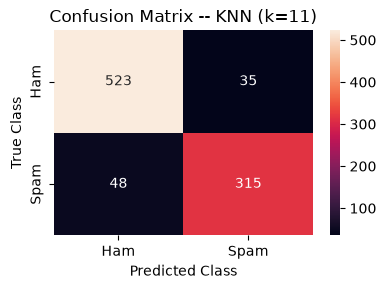
\includegraphics[width=0.7\linewidth]{images/knn_confusion_matrix.png}
\caption{Confusion Matrix — KNN (k=11)}
\end{figure}
\begin{figure}[H]
\centering
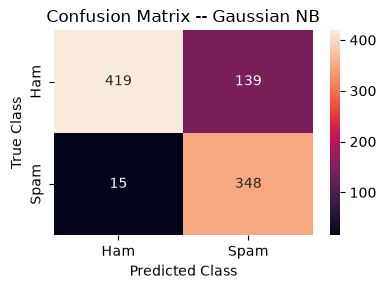
\includegraphics[width=0.7\linewidth]{images/gaussianNB_confusion_matrix.png}
\caption{Confusion Matrix — Gaussian NB}
\end{figure}
\begin{figure}[H]
\centering
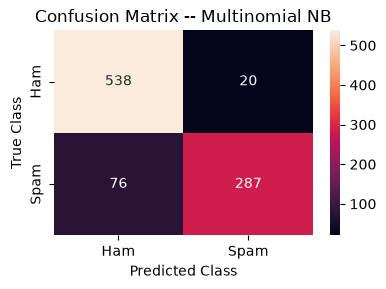
\includegraphics[width=0.7\linewidth]{images/multinomialNB_confusion_matrix.png}
\caption{Confusion Matrix — Multinomial NB}
\end{figure}
\begin{figure}[H]
\centering
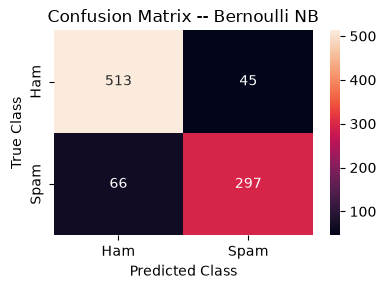
\includegraphics[width=0.7\linewidth]{images/bernoulliNB_confusion_matrix.png}
\caption{Confusion Matrix — Bernoulli NB}
\end{figure}

\textbf{Inference:}
TODO: Compare the confusion matrices across models — which model has fewer false positives / false negatives.

\subsection{Multi-Model ROC Curve Comparison}
\begin{figure}[H]
\centering
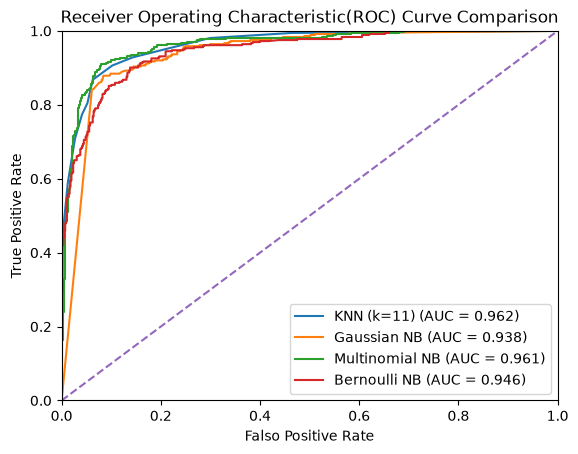
\includegraphics[width=0.7\linewidth]{images/multi_model_roc_comparison.png}
\caption{ROC Curve Comparison Across All Models}
\end{figure}

\textbf{Inference:}
TODO: Compare AUC scores — which model has the best discriminative ability.

\subsection{Time Comparison}
\begin{figure}[H]
\centering
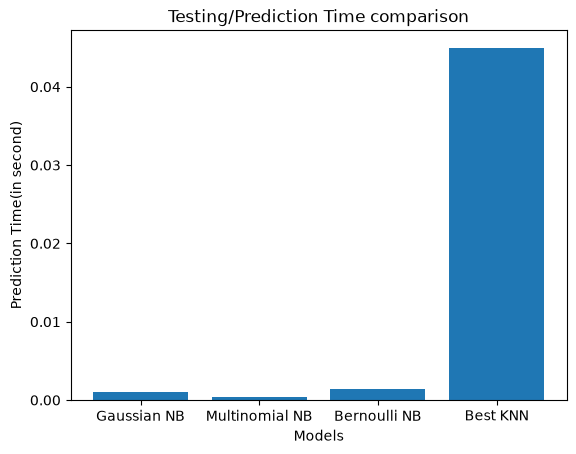
\includegraphics[width=0.7\linewidth]{images/prediction_time_comparison.png}
\caption{Prediction Time Comparison Across Models}
\end{figure}

\textbf{Inference:}
TODO: Discuss which model is fastest to predict.

\section{Results Comparison}
\begin{table}[H]
\centering
\begin{tabular}{lccccc}
\toprule
\textbf{Model} & \textbf{Accuracy} & \textbf{Precision} & \textbf{Recall} & \textbf{F1-Score} & \textbf{ROC-AUC} \\ \midrule
KNN (k=11) & 0.910 & 0.908 & 0.903 & 0.905 & TODO \\
Gaussian NB & 0.833 & 0.840 & 0.850 & 0.840 & 0.938 \\
Multinomial NB & 0.896 & 0.910 & 0.880 & 0.890 & 0.961 \\
Bernoulli NB & 0.879 & 0.880 & 0.870 & 0.880 & 0.946 \\
\bottomrule
\end{tabular}
\caption{Overall Performance Comparison Across All Models}
\end{table}

\section{Discussion}
TODO: Discuss observations, strengths, and limitations:
\begin{itemize}
    \item Which model performed best overall and why.
    \item Effect of scaling on different algorithms.
    \item Trade-off between accuracy and computational efficiency.
    \item Comparison of KNN tuning methods (GridSearchCV vs RandomizedSearchCV).
    \item KDTree vs BallTree performance differences.
    \item How Naive Bayes variants compare for this dataset.
\end{itemize}

\section{Conclusion}
TODO: Summarize the experiment — the application of KNN and Naive Bayes variants for email spam classification was demonstrated, with comparative analysis of performance metrics, confusion matrices, ROC curves, and time efficiency.

\section{References}
\begin{enumerate}
    \item TODO: Reference the Spambase dataset (UCI Repository).
    \item TODO: Reference scikit-learn documentation for KNN and Naive Bayes.
    \item TODO: Reference pandas, Matplotlib, and Seaborn documentation.
\end{enumerate}

\end{document}